\documentclass[tikz,border=3pt]{standalone}
\usepackage{pgfplots}
\usepgfplotslibrary{groupplots}
\pgfplotsset{compat=1.17}
\definecolor{pdcsblue}{RGB}{0,114,178}
\definecolor{pdcsorange}{RGB}{213,94,0}
\begin{document}
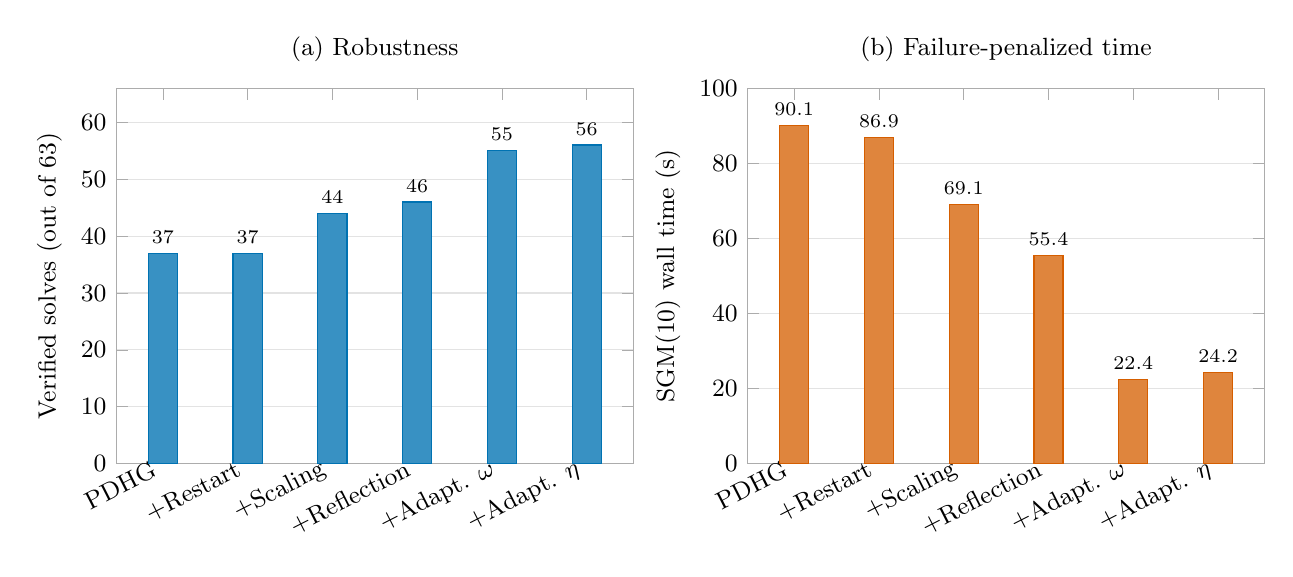
\begin{tikzpicture}
\begin{groupplot}[
  group style={group size=2 by 1,horizontal sep=1.45cm},
  width=8.15cm,
  height=6.35cm,
  xmin=0.45,
  xmax=6.55,
  xtick={1,2,3,4,5,6},
  xticklabels={PDHG,+Restart,+Scaling,+Reflection,+Adapt. $\omega$,+Adapt. $\eta$},
  xticklabel style={rotate=27,anchor=east,font=\small},
  tick label style={font=\small},
  label style={font=\small},
  title style={font=\small},
  ymajorgrids=true,
  grid style={gray!22},
  axis line style={gray!65},
  tick style={gray!65},
  enlarge x limits=false,
]
\nextgroupplot[
  title={(a) Robustness},
  ylabel={Verified solves (out of 63)},
  ymin=0,
  ymax=66,
  ytick={0,10,20,30,40,50,60},
]
\addplot[
  ybar,
  bar width=10.5pt,
  fill=pdcsblue!78,
  draw=pdcsblue,
  line width=0.45pt,
  point meta=y,
  nodes near coords,
  every node near coord/.append style={font=\scriptsize},
] coordinates {(1,37) (2,37) (3,44) (4,46) (5,55) (6,56)};

\nextgroupplot[
  title={(b) Failure-penalized time},
  ylabel={SGM(10) wall time (s)},
  ymin=0,
  ymax=100,
  ytick={0,20,40,60,80,100},
]
\addplot[
  ybar,
  bar width=10.5pt,
  fill=pdcsorange!76,
  draw=pdcsorange,
  line width=0.45pt,
  point meta=y,
  nodes near coords={
    \pgfmathprintnumber[fixed,precision=1]{\pgfplotspointmeta}
  },
  every node near coord/.append style={font=\scriptsize},
] coordinates {(1,90.127627) (2,86.865183) (3,69.087108) (4,55.408437) (5,22.40793) (6,24.224281)};
\end{groupplot}
\end{tikzpicture}
\end{document}
